%%%%%%%%%%%%%%%%%%%%%%%%%% ch2-StochasticProcess
\begin{frame}[shrink]
\frametitle{ch2.信号检测与估计理论的基础知识}
\tableofcontents[hideallsubsections]
\end{frame}

\section{随机过程的定义}

\begin{frame}{随机过程引例(1)}
\begin{example}
	考察$[0,t_0]$时间内某网站收到的访问次数$X(t_0)$, $X(t_0)$则是一个随机变量。
	\begin{itemize}
		\item 如果要长时间内该网站的访问次数,则需要让$t$变化起来,即$t$趋于无穷大,则$X(t)$是一簇随机变量.
		\item 此时$X(t)$是与时间有关系的随机变量, 称$\{X(t),t\in[0,\infty]\}$是随机过程。
	\end{itemize}	
\end{example}
\end{frame}

\begin{frame}{随机过程引例(1)}
\begin{example}
	具有随机初位相的简谐波
	\[X(t)=A\cos(\omega t+\Phi)\]
	其中$A,\omega$为常数,$\Phi$服从$[0,2\pi]$上的均匀分布。
	\begin{itemize}
		\item 由于初位相的随机性,在某时刻$t=t_0,X(t)$是一个随机变量.
		\item 若要观察任一时刻$t$的波形,则需要用一簇随机变量$X(t)$描述. 
		\item 称$\{X(t),t\in[0,\infty]\}$是随机过程。
	\end{itemize}	
\end{example}
\end{frame}

\begin{frame}{随机过程引例(2)}
\begin{columns}
	\column{0.6\textwidth}
	\begin{example}
		三次热噪声电压测量结果:固定$t$时刻电压,对应一个随机变量$v(t)$; 无限个$t$,则无限个电压---时间的函数族构成一随机过程。
	\end{example}
	\column{0.4\textwidth}
	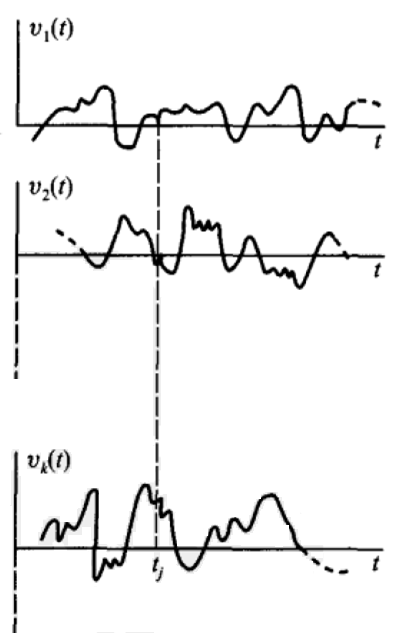
\includegraphics[scale=0.4]{vt}
\end{columns}
\end{frame}

\begin{frame}{随机过程引例(3)}
\begin{example}
	生物群体的增长问题.以$X_t$表示在时刻$t$某种生物群体的个数,则对每一个固定的$t,X_t$是一个随机变量。 
	\begin{itemize}
		\item 如果从$t=0$开始,每隔24小时对群体的个数观察一次,则对每一个$t$,$X_t$是一簇随机变量。记为$X_n,n=0,1,\dots$
		\item 若要观察任一时刻$t$的波形,则需要用一族随机变量$X(t)$描述. 
		\item 称$\{X_t,t=0,1,2,\dots\}$是随机过程。
	\end{itemize}	
\end{example}
\end{frame}

\begin{frame}{随机过程引例特点}
\begin{block}{以上例子的共同特点---随机现象在时间上的延展$\implies$随机过程}
	\begin{itemize}
		\item 给定一个$t$,就有一个随机变量$X(t)$与之对应。
		\item 概率论主要是以\textbf{一个或有限个随机变量}为研究对象的.
		\item 随机过程是概率论的``动力学''部分,研究对象为随时间演变的随机现象,通常会有\textbf{无穷多个随机变量}。
	\end{itemize}	
\end{block}
\end{frame}

\begin{frame}%{随机过程的定义}
\begin{definition}[随机过程]
	设$(\Omega,\mathcal{F},P$是一概率空间, $T$是一实参数集,定义在$\Omega$和$T$上的二元函数$x(t,\xi)$
	\begin{enumerate}
		\item 固定$t_k\in T,x(t_k,\xi)$是概率空间上的随机变量;
		\item 固定$\xi_i\in\Omega,x(t,\xi_i)$是概率空间上的随机函数(或称$x(t,\xi_i)$是对应于$\xi_i$的样本函数)
	\end{enumerate}
    则称$\{x(t,\xi),t\in T,\xi\in \Omega \}$为一随机过程,简记为$x(t)$,其中$t$和$\xi$均是变量。\\
	随机过程的定义域是实参数集$T$和样本空间$\Omega$。值域是$\mathbb{R}$.
	\begin{itemize}
		\item 样本空间$\Omega$:一个随机试验所有可能出现的结果的全体,称为随机事件的样本空间。\\
		\item 事件域$\mathcal{F}$: 样本空间中的某些子集。
		\item
		参数集$T$表示时间或空间,通常的形式: $T=\{0,1,2,\dots \}$或$T=[a,b],T=[-\infty,\infty]$
	\end{itemize}
	\end{definition}
\end{frame}

\begin{frame}
用映射表示随机过程: 
\[x(t,\xi): T\times\Omega\to\mathbb{R} \]
\begin{enumerate}
	\item $x(t,\xi)$实质是定义在$T\times\Omega$上的二元单值函数;
	\item 固定$t\in T,x(t,\cdot)$是样本空间$\Omega$上的函数,即为一随机变量;
	\item 固定$\xi_i\in\Omega,x(\cdot,\xi_i)$是一个关于$t\in T$的函数,通常称为样本函数,或称随机过程的一次实现,所有样本函数的集合确定一随机过程。
	\item 随机过程$\{x(t,\xi)\}$可能取值的全体所构成的集合称为此随机过程的状态空间,记作$S$。$S$中的元素称为状态。状态空间可以由复数、实数或更一般的抽象空间构成。
\end{enumerate}
\end{frame}

\begin{frame}
\begin{example}[随机过程示例]
	抛掷硬币的试验,样本空间$\Omega=\{H,T\}$, 定义
	\[x(t)=\begin{cases}
	\cos\pi t, &\text{当出现$H$}\\
	t, &\text{当出现$T$}\\ 
	\end{cases}, t\in(-\infty,\infty)\]
	其中$P(H)=P(T)=1/2$
\end{example}
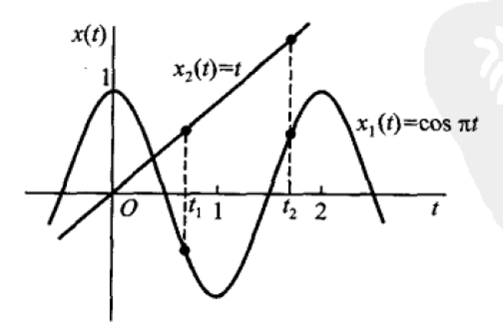
\includegraphics[scale=0.5]{sin_t}
\end{frame}

\begin{frame}
\begin{example}
	考察$[0,t_0]$时间内某网站收到的访问次数$X(t_0)$, $X(t_0)$则是一个随机变量。
	\begin{itemize}
		\item 如果要长时间内该网站的访问次数,则需要让$t$变化起来,即$t$趋于无穷大,则$X(t)$是一簇随机变量.
		\item 此时$X(t)$是与时间有关系的随机变量, 称$\{X(t),t\in[0,\infty]\}$是随机过程。
	\end{itemize}
\end{example}
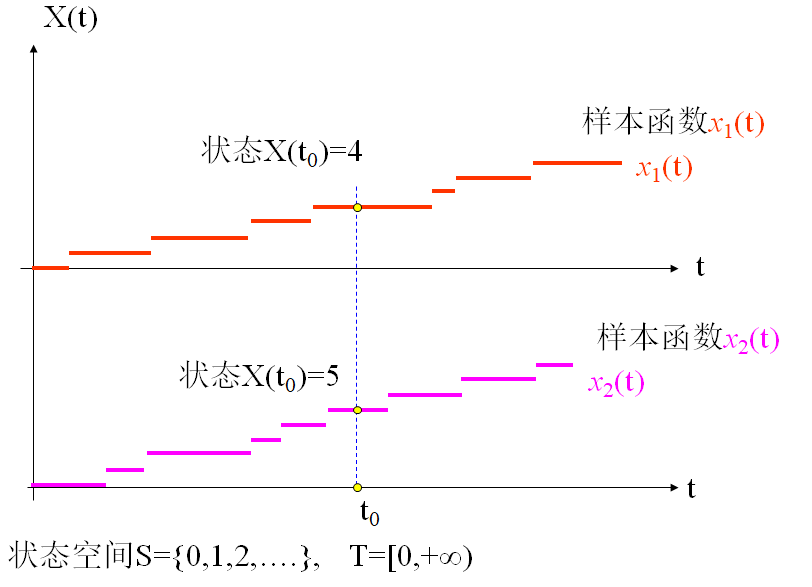
\includegraphics[scale=0.2]{sampleFun1}	
\end{frame}

\begin{frame}
\begin{example}
具有随机初位相的简谐波
\[X(t)=A\cos(\omega t+\Phi)\]
其中$A,\omega$为常数,$\Phi$服从$[0,2\pi]$上的均匀分布。
\begin{itemize}
	\item 由于初位相的随机性,在某时刻$t=t_0,X(t)$是一个随机变量.
	\item 若要观察任一时刻$t$的波形,则需要用一簇随机变量$X(t)$描述. 
	\item 称$\{X(t),t\in[0,\infty]\}$是随机过程。
\end{itemize}	
\end{example}
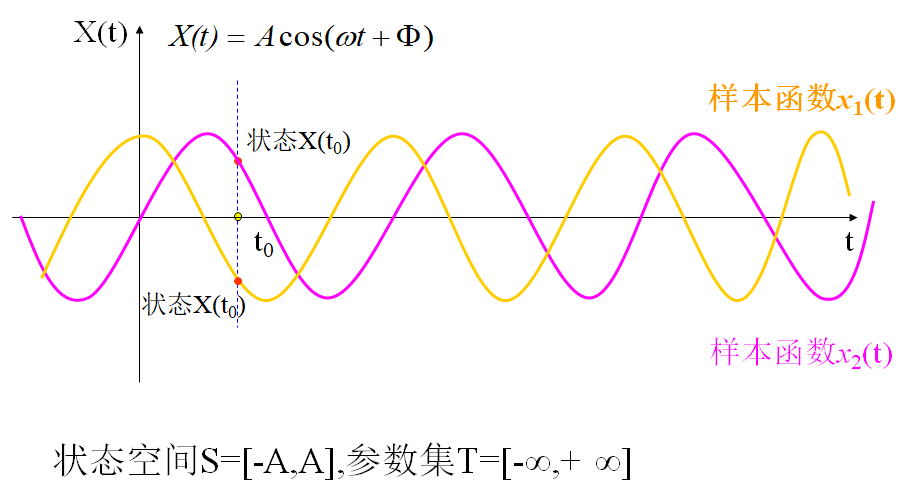
\includegraphics[scale=0.2]{sampleFun2}	
\end{frame}

\begin{frame}
\begin{columns}
\column{0.6\textwidth}
\begin{example}
三次热噪声电压测量结果:固定$t$时刻电压,对应一个随机变量$v(t)$; \\
无限个$t$,则无限个电压---时间的函数族构成一随机过程。\\
~\\
样本函数$\implies$
\end{example}
\column{0.4\textwidth}
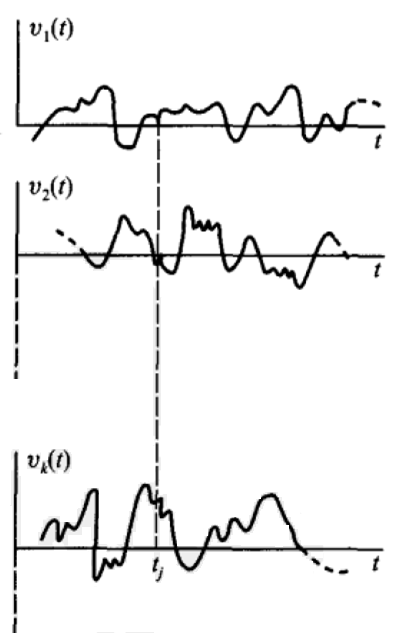
\includegraphics[scale=0.4]{vt}
\end{columns}
\end{frame}

\begin{frame}
\begin{example}
生物群体的增长问题.以$X_t$表示在时刻$t$某种生物群体的个数,则对每一个固定的$t,X_t$是一个随机变量。 
\begin{itemize}
\item 如果从$t=0$开始,每隔24小时对群体的个数观察一次,则对每一个$t$,$X_t$是一簇随机变量。记为$X_n,n=0,1,\dots$
\item 若要观察任一时刻$t$的波形,则需要用一族随机变量$X(t)$描述. 
\item 称$\{X_t,t=0,1,2,\dots\}$是随机过程。
\end{itemize}	
\end{example}
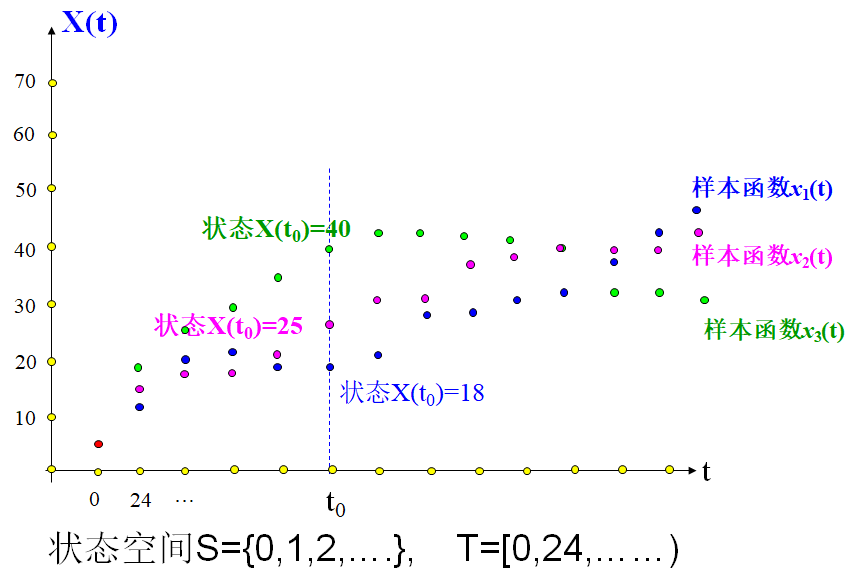
\includegraphics[scale=0.15]{sampleFun3}	
\end{frame}

\section{随机过程的统计描述}

\begin{frame}
连续随机过程$\{x(t,\xi),t\in T,\xi\in\Omega \}$的$M$个样本函数如图。通常用有限维概率密度函数来描述随机过程。
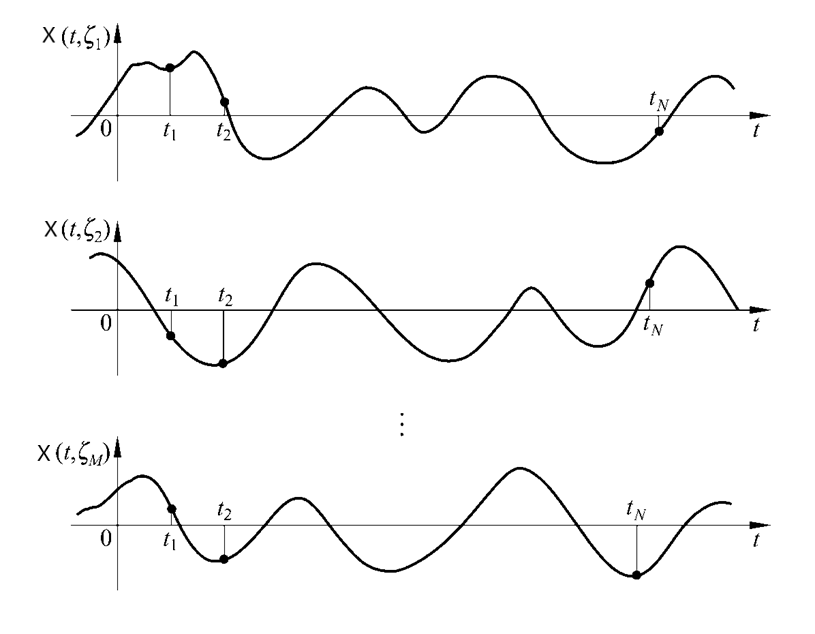
\includegraphics[scale=0.5]{sampleFun}
\end{frame}

\begin{frame}
设$\{x(t,\xi),t\in T,\xi\in\Omega \}$是一随机过程,对于任意固定的时刻$t,x(t,\xi)$是一随机变量,称
\[F(x;t)=P\{x(t,\xi)\le x\},x\in\mathbb{R},t\in T \]
为该随机过程的一维累积分布函数。如果$F(x;t)$对$x$的一阶导数存在,则有
\[p(x;t)=\frac{dF(x;t)}{dx}\]
$p(x;t)$称为随机过程$x(t,\xi)$的一维概率密度函数。
\end{frame}

\begin{frame}
对于任意固定的时刻$t_1,t_2\in T$, 随机变量$x(t_1,\xi),x(t_2,\xi)$构成二维矢量$[x(t_1,\xi),x(t_2,\xi)]^T$,称
\[F(x_1,x_2;t_1,t_2)=P\{x(t_1,\xi)\le x_1,x(t_2,\xi)\le x_2\},x_1,x_2\in\mathbb{R},t_1,t_2\in T \]
为该随机过程的二维累积分布函数。如果$F(x_1,x_2;t_1,t_2)\in T$对$x_1,x_2$的二阶混合偏导数存在,则有
\[p(x_1,x_2;t_1,t_2)=\frac{\partial^2 F(x_1,x_2;t_1,t_2)}{\partial x_1\partial x_2}\]
$p(x;t)$称为随机过程$x(t,\xi)$的二维联合概率密度函数。
\end{frame}

\begin{frame}
推广至N维随机矢量的情况\\
随机过程的N维累积分布函数
\begin{align*}
F(x_1,x_2,\cdots,x_N;t_1,t_2,\cdots,t_N)&=\\
&P\{x(t_1,\xi)\le x_1,x(t_2,\xi),\cdots,x(t_N,\xi)\le x_N\},&\\
&x_1,x_2,\cdots,x_N\in\mathbb{R},t_1,t_2,\cdots,t_N\in T
\end{align*}
随机过程的N维联合概率密度函数
\begin{align*}
p(x_1,x_2,\cdots,x_N;t_1,t_2,\cdots,t_N)&=\\
&\frac{\partial^N F(x_1,x_2,\cdots,x_N;t_1,t_2,\cdots,t_N)}{\partial x_1\partial x_2\cdots\partial x_N}
\end{align*}
\end{frame}

\begin{frame}{雅可比变换法}
设一维随机变量为$x(\xi)$,它的概率密度函数$p(x)$已知,若$x(\xi)$的一个函数为
\[y(\xi)=g(x(\xi)) \]
该函数也是一维随机变量。若它的反函数存在,即有
\[x(\xi)=h(y(\xi)) \]
且连续可导,则$y(\xi)$的概率密度函数为
\[p(y)=p[x=h(y)]|J| \]
这种变换称为一维雅可比变换,其中雅可比$J=\frac{dh(y)}{dy}$, $|\bullet|$是绝对值符号。
\end{frame}

\begin{frame}
\begin{example}
	设随机过程$x(t)=V\cos\omega t,t\in(-\infty,+\infty)$, 其中$\omega$为常数, $V$服从$[0,1]$上的均匀分布。
	\begin{enumerate}
		\item 确定$\{x(t),t\in(-\infty,+\infty)\}$的两个样本函数。
		\item 求$t=0,t=3\pi/4\omega$时,随机变量的概率密度函数。
		\item 求$t=\pi/2\omega$时, $x(t)$的分布函数。
	\end{enumerate}
\end{example}
\end{frame}

\begin{frame}
解:
\begin{enumerate}
	\item 取$V=1/2,1/3$分别得到两个样本函数
	\[x_1(t)=\frac{1}{2}\cos\omega t,x_2(t)=\frac{1}{3}\cos\omega t\]
	\item $t=0$时,$x(t)=V\cos\omega 0=V$,而$V$为$[0,1]$上的均匀分布,则
	$$
	p(x;t=0)=\begin{cases}
	1 & 0\le x\le 1\\
	0 &\text{其它}
	
\end{cases}
$$
\end{enumerate}
\end{frame}

\begin{frame}
解(续):
\begin{enumerate}
	\setcounter{enumi}{1} %设定起始编号 
	\item (续) 当$t=\frac{3\pi}{4\omega}$时,$x(t)=V\cos\omega\frac{3\pi}{4\omega}=-\frac{\sqrt{2}}{2}V$
	由于函数$x=-\frac{\sqrt{2}}{2}V$的反函数为$V=h(x)=-\sqrt{2}x$,其导数为$h^\prime(x)=-\sqrt{2}$,则利用一维雅可比变换公式,求得
	\begin{align*}
		p(x,t=\frac{3\pi}{4\omega}) &=\begin{cases}
		p_V(h(x))|h^\prime(x)| &0\le h(x)\le 1\\
		0 &\text{其它}
		\end{cases}\\
		&=\begin{cases}
		\sqrt{2} &0\le -\sqrt{2}x\le 1\\
		0 &\text{其它}
		\end{cases}\\
		&=\begin{cases}
		\sqrt{2} &\frac{-\sqrt{2}}{2}\le x\le 0\\
		0 &\text{其它}
		\end{cases}
	\end{align*}
\end{enumerate}
\end{frame}

\begin{frame}
解(续):
\begin{enumerate}
	\setcounter{enumi}{2} %设定起始编号 
	\item $t=\frac{\pi}{2\omega}$时,$x(t)=V\cos\omega\frac{pi}{2\omega}=0$, 此时$x(t=\frac{\pi}{2\omega})$是单点分布,则
	\begin{align*}
	F(x,t=\frac{\pi}{2\omega}) &=P\{x(t)\le x \}\\
	&=\begin{cases}
	1 &x\ge 0\\
	0 &x<0
	\end{cases}
	\end{align*}
\end{enumerate}
\end{frame}

\begin{frame}
\begin{example}
	设随机相位正弦信号$s(t;\theta)=a\cos(\omega_0 t+\theta)$, 其中振幅$a$和$\omega_0$为常数, 相位$\theta$是一随机变量,它服从$(-\pi,\pi)$上的均匀分布。
	\begin{enumerate}
		\item 求该过程的均值和自相关函数。
		\item 写出$x(t;\theta)$的样本函数。
		\item 求$x(t;\theta)$的概率密度函数。
	\end{enumerate}
\end{example}
\end{frame}

\begin{frame}
解:
\begin{enumerate}
	\item 因为相位$\theta$服从$(-\pi,\pi)$上的均匀分布,所以,
	$$p(\theta)=\begin{cases}
	\frac{1}{2\pi}, & -\pi\le\theta\le\pi\\
	0, &\text{其它}
	\end{cases} $$ 
	该随机过程的均值为:
	\begin{align*}
	\mu_x(t)&=E[s(t;\theta)]=E[a\cos(\omega_0t+\theta)]\\
	&=\int_{-\infty}^{\infty}a\cos(\omega_0t+\theta)p(\theta)d\theta\\
	&=\int_{-\pi}^{\pi}a\cos(\omega_0t+\theta)\frac{1}{2\pi}d\theta\\
	&=\frac{a}{2\pi}\int_{-\pi}^{\pi}\cos(\omega_0t+\theta)d\theta\\
	&=0
	\end{align*}
\end{enumerate}
\end{frame}

\begin{frame}
解(续):
\begin{enumerate}
	\item (续) 该随机过程的自相关函数为:
	\begin{align*}
	\r_x(t_j,t_k)&=E[x(t_j)x(t_k)]\\
	&=\int_{-\infty}^{\infty}a\cos(\omega_0t_j+\theta)a\cos(\omega_0t_k+\theta)p(\theta)d\theta\\
	&=\frac{a^2}{4\pi}\int_{-\pi}^{\pi}[\cos(\omega_0t_j+\omega_0t_k+2\theta)+\cos\omega_0(t_k-t_j)]d\theta\\
	&=\frac{a^2}{2}\cos\omega_0\tau,\qquad(\tau=t_k-t_j)
	\end{align*}
	\item 当$\theta$在$(-\pi,\pi)$内任取定值时,如$\theta=0$, 则样本函数为
	$$x(t;\theta=0)=a\cos\omega_0t$$
	当$\theta=\frac{\pi}{2}$, 则样本函数为
	$$x(t;\theta=\frac{\pi}{2})=a\cos(\omega_0t+\frac{\pi}{2})=-a\sin\omega_0t$$
\end{enumerate}
\end{frame}

\begin{frame}
解(续):
\begin{enumerate}
	\setcounter{enumi}{2} %设定起始编号 
	\item 求$x(t;\theta)$的概率密度函数。\\
	固定时刻$t$, 则随机变量$x(t;\theta)=a\cos(\omega_0t+\theta)$是随机变量$\theta$的函数。
	由分布函数的定义:
	$$F_{x(t)(y)}=P\{x(t)\le y\}=P\{a\cos(\omega_0t+\theta)\le y \}$$
	当$y<-a$时,$F_{x(t)(y)}=0$; 当$y\ge +a$时, $F_{x(t)}(y)=1$\\
	当$-a<y\le +a$时,我们有:
	\begin{align*}
	F_{x(t)}(y) &=P\{x(y)\le y \}=P\{a\cos(\omega_0t+\theta)\le y \}\\
	&=P(\{-\pi<\theta\le\omega_0t-\arccos\frac{y}{a} \} \cup \{\arccos\frac{y}{a}-\omega_0t<\theta\le\pi \})\\
	&=\frac{1}{2\pi}\left[\int_{-\pi}^{\omega_0t-\arccos\frac{y}{a}}dx+\int_{\arccos\frac{y}{a}-\omega_0t}^{\pi}dx\right]\\
	&=\frac{1}{\pi}[\omega_0t+\pi-\arccos\frac{y}{a}]
	\end{align*}	
\end{enumerate}
\end{frame}

\begin{frame}
解(续):
\begin{enumerate}
	\setcounter{enumi}{2} %设定起始编号 
	\item 求$x(t;\theta)$的概率密度函数。\\
	当$-a<y\le +a$时, 有: $F_{x(t)}(y)=\frac{1}{\pi}[\omega_0t+\pi-\arccos\frac{y}{a}]$\\
	此时, $x(t;\theta)$的概率密度函数为:
	$$p_{x(t)}(y)=F_{x(t)}^\prime(y)=\frac{1}{\pi\sqrt{a^2-y^2}} $$
	最终得到$x(t;\theta)$的概率密度函数为:
	$$ p(\theta;t)=
	\begin{cases}
		\frac{1}{\pi\sqrt{a^2-x^2}}, &-a<x\le +a \\
		0,&\text{其它}
	\end{cases}
	$$
\end{enumerate}
\end{frame}

\section{狄拉克函数(Dirac函数/$\delta$函数)}

\begin{frame}{狄拉克函数(Dirac函数/$\delta$---函数)}
\begin{definition}[$\delta$---函数]
	对于任意的无穷次可微的函数$f(t)$, 如果满足:
	$$\int_{-\infty}^{\infty}\delta (t)f(t)dt=\lim\limits_{\varepsilon\to 0}\int_{-\infty}^{\infty}\delta_{\varepsilon}(t)f(t)dt $$
	其中:
	\[
	\delta_{\varepsilon}(t)=\begin{cases}
	0,&t<0\\
	\frac{1}{\varepsilon}, & 0\ge t<\varepsilon\\
	0, &t>\varepsilon
	\end{cases}
	\]
	则称$\delta_\varepsilon(t)$的弱极限为$\delta$函数,记为$\delta(t)$
	显然, 对于任意的$\varepsilon>0$, 有:
	$$\int_{-\infty}^{\infty}\delta_{\varepsilon}(t)dt=\int_{-\infty}^\infty\frac{1}{\varepsilon}dt=1\implies \int_{-\infty}^\infty\delta(t)dt=1$$
\end{definition}
\end{frame}

\begin{frame}{狄拉克函数(Dirac函数/$\delta$---函数)}
\begin{block}{注}
	\begin{enumerate}
		\item $\delta(t)$在$t=0$点的取值为$\infty$, 在$t\ne 0$点的取值为0, 并且满足$\int_{-\infty}^{\infty}\delta(t)dt=1$。
		\item 工程(信号处理等)上$\delta$---函数也称为单位脉冲或单位冲激函数。
	\end{enumerate}
\end{block}
\begin{block}{$\delta$---函数的筛选性质}
	若$f(t)$为无穷此可微的函数,则有:$\int_{I}\delta(t)f(t)dt=f(0) $\\
	其中$I$是包含点$t=0$的任意区间。特殊地, 有:$\int_{-\infty}^{\infty}\delta(t)f(t)dt=f(0) $\\
	更一般地,我们有:
	$$\int_{-\infty}^{\infty}\delta(t-t_0)f(t)dt=f(t_0) $$
\end{block}
\end{frame}

\begin{frame}[shrink]
\frametitle{离散型随机变量分布列的$\delta$---函数表示}
设离散型随机变量$X$的分布列为: $P\{X=x_i\}=p_i,i=1,2,\dots$, 则由$\delta$---函数的筛选性质可以定义离散型随机变量$X$的概率密度函数为:
$$p(x)=\sum\limits_{i=0}^{\infty}p_i\delta(x-x_i)$$
因为,由$\delta$---函数的筛选性质,离散型随机变量$X$的分布函数可以表示为:
$$F(x)=P\{X\le x\}=\sum\limits_{x_i\le x}p_i=\int_{-\infty}^{x}\sum\limits_{i=1}^{\infty}p_i\delta(u-x_i)du$$
\begin{columns}
	\column{0.6\textwidth}
	\begin{block}{}
		工程上,常用离散型随机变量分布列的$\delta$---函数表示法,将离散型随机变量的分布列表示成概率密度函数的形式,因此与连续型随机变量的概率分布密度函数一样进行统一处理。
	\end{block}
	\column{0.3\textwidth}
	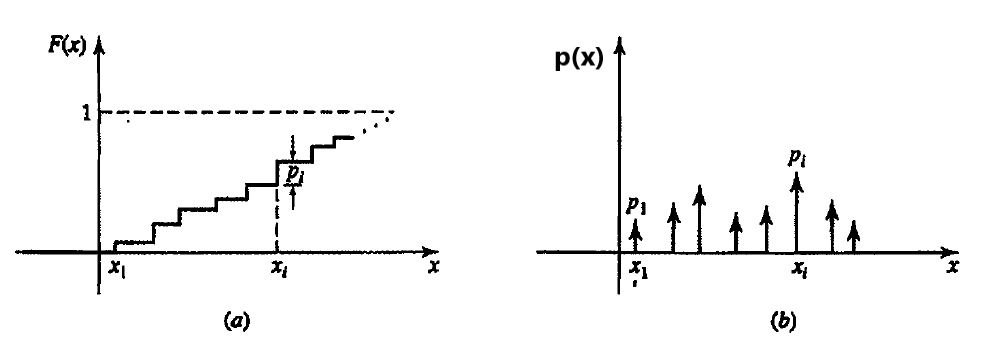
\includegraphics[scale=0.15]{pi}\\
	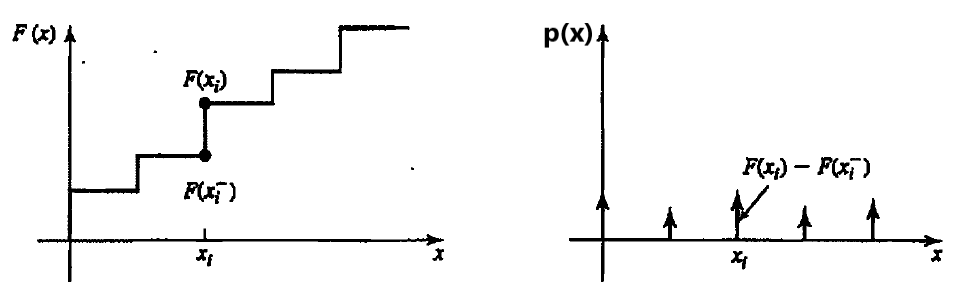
\includegraphics[scale=0.15]{Fx-px}
\end{columns}
\end{frame}

\begin{frame}
\begin{example}
设有一采用脉宽调制以传输信息的通信系统。脉冲的重复周期为$T$,每个周期传输一个值, 脉冲宽度收到随机信息的调制,使每个脉冲的宽度$\tau$服从$(0,T)$上的均匀分布,而且不同周期的脉宽是相互统计独立的随机变量。脉冲的幅度为常数$A$。 也就是说,这个通信系统传送的信号是随机脉宽等幅度的周期信号,它是一个随机过程。下图画出了它的一个样本函数。试求该随机过程$x(t)$的一维概率密度函数。
\begin{figure}
	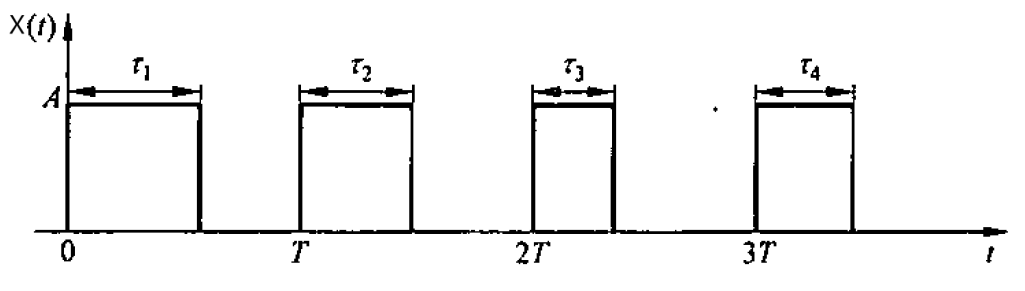
\includegraphics[scale=0.3]{2_10SampleFun}
	\caption {脉宽调制信号的一个样本函数}
\end{figure}
\end{example}
\end{frame}

\begin{frame}
\begin{example}[解]
	因为脉冲的重复周期为$T$,所以只需求出一个周期的概率密度函数。\\
	在一个周期内,随机信号为
	\[
	x(t)=\begin{cases}
	A,&t\le\tau\\
	0,&\tau<t\le T
	\end{cases} 
	\]
	$x(t)$的分布函数为
	\[
	F(x;t)=\begin{cases}
	0,&x<0\\
	\frac{t}{T},&0\ge x<A\\
	1,&x\ge A
	\end{cases} 
	\]
	所以,它的一维概率密度函数为:
	\[p(x;t)=\frac{t}{T}\delta(x)+(1-\frac{t}{T})\delta(x-A) \]
\end{example}
\end{frame}

%\section{随机过程的统计平均量}

\begin{frame}
函数的均值
\[\bar{y}=\frac{1}{b-a}\lim\limits_{\Delta x\to 0}\sum\limits_{i=1}^{n}f(x_{i-1})\Delta x=\frac{1}{b-a}\int_{a}^{b}f(x)dx \]
交流电$i=I_m\sin\omega t$,电压$u=iR=I_mR\sin\omega t$,功率$p=ui=I_m^2R\sin^2\omega t$\\
此功率在长度为一个周期的区间$[0,\frac{2\pi}{\omega}]$上的平均值
\[\bar{p}=\frac{1}{\frac{2\pi}{\omega}}\int_{0}^{\frac{2\pi}{\omega}}I_m^2R\sin^2\omega tdt=\frac{I_m^2R}{2}=\frac{I_mU_m}{2},(U_m=I_mR) \]
$I_m,U_m$为交流电电流、电压的最大值,$\omega$为交流电的角频率。
\end{frame}

\begin{frame}
\begin{block}{随机过程的均值$\mu_x(t)$: 表示随机过程在$t$时刻状态取值的理论平均值}
	\[\mu_x(t)\mathop{=}^{def}E[x(t)]=\int_{-\infty}^{\infty}xp(x;t)dx \]
	如果$x(t)$是电压或电流,则$\mu_x(t)$可以理解为在$t$时刻的``直流分量''。
\end{block}

\begin{block}{随机过程的均方值$\varphi_x^2(t)$}
	\[\varphi_x^2(t)\mathop{=}^{def}E[x^2(t)]=\int_{-\infty}^{\infty}x^2p(x;t)dx \]
	如果$x(t)$是电压或电流,则$\varphi_x^2(t)$可以理解在$t$时刻它在$1\Omega$电阻上消耗的``平均功率''。
\end{block}
\end{frame}

\begin{frame}
\begin{block}{随机过程的方差/标准偏差$\delta_x^2(t)$}
\[\sigma_x^2(t)\mathop{=}^{def}E[(x(t)-\mu_x(t))^2]=\int_{-\infty}^{\infty}(x-\mu_x(t))^2p(x;t)dx \]
方差$\sigma_x^2(t)$表示随机过程在$t$时刻取其值偏离其均值$\mu_x(t)$的离散程度。如果$x(t)$是电压或电流,则$\delta_x^2(t)$可以理解在$t$时刻它在$1\Omega$电阻上消耗的``交流功率''。
\end{block}
\begin{block}{均值$\mu_x(t)$,均方值$\varphi_x^2(t)$,方差$\delta_x^2(t)$之间的关系}
\[\sigma_x^2(t)=\varphi_x^2(t)-\mu_x^2(t)\]
\end{block}
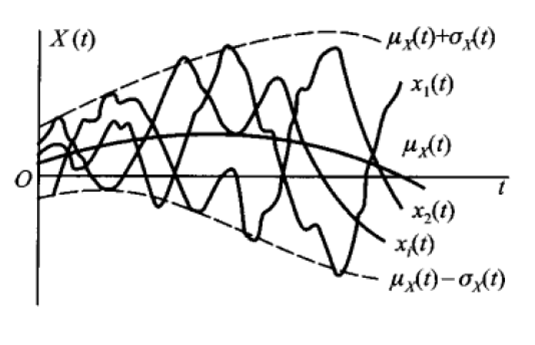
\includegraphics[scale=0.4]{delta}
\end{frame}

\begin{frame}
\begin{block}{随机过程的自相关函数$r_x(t_j,t_k)$}
\begin{align*}
r_x(t_j,t_k)&\mathop{=}^{def}E[x(t_j)x(t_k)]\\
&=\int_{-\infty}^{\infty}	\int_{-\infty}^{\infty}x_jx_kp(x_j,x_k;t_j,t_k)dx_jdx_k
\end{align*}
\end{block}
随机过程的自相关函数$r_x(t_j,t_k)$可以理解为它的两个随机变量$x(t_j)$与$x(t_k)$之间含有均值时的相关程度的度量。显然
\[r_x(t,t)=\varphi_x^2(t)\]
\end{frame}

\begin{frame}
\begin{block}{随机过程的自协方差函数$c_x(t_j,t_k)$}
\begin{align*}
c_x(t_j,t_k)&\mathop{=}^{def}E[((x(t_j)-\mu_x(t_j)(x(t_k)-\mu_x(t_k)]\\
&=\int_{-\infty}^{\infty}\int_{-\infty}^{\infty}(x_j-\mu_x(t_j))(x_k-\mu_x(t_k))p(x_j,x_k;t_j,t_k)dx_idx_k
\end{align*}
\end{block}
随机过程的自协方差函数$c_x(t_j,t_k)$可以理解为它的两个随机变量$x(t_j)$与$x(t_k)$之间的相关程度的度量。它们的自相关系数定义为
\[\rho_x(t_j,t_k)\mathop{=}^{def}\frac{c_x(t_j,t_k)}{\sigma_x(t_j)\sigma_x(t_k)}\]
易证
\[c_x(t_j,t_k)=r_x(t_j,t_k)-\mu_x(t_j)\mu_x(t_k)\]
\[c_x(t,t)=\sigma_x^2(t)\]
\end{frame}

\begin{frame}
\begin{example}
	考察一随机过程,它在$t_0+nT_0$时刻具有宽度为b的矩形脉冲波,脉冲幅度为一等概率$(p)$,取值$\pm a$的随机变量,且$b<T_0,T_0$是在$(0,T_0)$上服从均匀分布的随机变量,并且脉冲幅度$A$与$t_0$独立, 试求该过程的自相关函数和方差。
\end{example}
解: 由给定的随机过程,我们有,均值: 
$$\mu_x(t)=E\{x(t)\}=a\times p+(-a)\times p + 0\times(1-2p)=0$$
下面求自相关函数:\\
任取$t_1,t_2$,且$t_1<t_2$,当$|t_1-t_2|>T_0$时, $t_1,t_2$位于不同的周期内,此时有:
$$r_x(t_1,t_2)=E\{x(t_1)x(t_2)\}=E\{x(t_1)\}E\{x(t_2)\}=0$$

当$|t_1-t_2|\le T_0$, 且$t_1,t_2$位于两个不同的周期内时,此时有:
$$r_x(t_1,t_2)=E\{x(t_1)x(t_2)\}=E\{x(t_1)\}E\{x(t_2)\}=0$$
\end{frame}

\begin{frame}
当$|t_1-t_2|\le T_0$, 且$t_1,t_2$位于同一周期内时,假设$\theta$为$t_1$所在的脉冲的起始时刻,只有当$t_2<\theta+b$时, $x(t_1)和x(t_2)$取到不为0的值, 此时的概率为:
$$P\{t_2<\theta+b \}=1-P\{t_2>\theta+b\}=1-\frac{1}{T_0}\int_{t_1-T_0}^{t_2-b}d\theta=\frac{b-(t_2-t_1)}{T_0}$$
由此,我们有:
$$r_x(t_1,t_2)=E\{x(t_1)\}E\{x(t_2)\}=a^2\cdot\frac{b-(t_2-t_1)}{T_0}$$
同理,当$t_1>t_2$时,我们有:
$$r_x(t_1,t_2)=E\{x(t_1)x(t_2)\}=a^2\cdot\frac{b-(t_1-t_2)}{T_0}$$
因此,最终得到自相关函数和方差:
$$r_x(\tau)=\frac{a^(b-|\tau|)}{T_0},\tau=t_2-t_1,\qquad \sigma_x^2(t)=r_x(0)=\frac{a^2b}{T_0}$$
\end{frame}

\begin{frame}
\begin{block}{随机过程的互相关函数$r_{xy}(t_j,t_k)$}
\begin{align*}
r_{xy}(t_j,t_k) &\mathop{=}^{def}E[x(t_j)y(t_k)]\\
&=\int_{-\infty}^{\infty}\int_{-\infty}^{\infty}x_jy_kp(x_j,t_j;y_k,t_k)dx_jdy_k
\end{align*}
式中, $p(x_j,t_j;y_k,t_k)$是$x(t)$与$y(t)$的二维混合概率密度函数。
\end{block}
\end{frame}

\begin{frame}
\begin{block}{随机过程的互协方差函数$c_{xy}(t_j,t_k)$}
\begin{align*}
c_{xy}(t_j,t_k)&\mathop{=}^{def}E[(x(t_j)-\mu_x(t_j))(y(t_k)-\mu_x(t_k))]\\
&=\int_{-\infty}^{\infty}\int_{-\infty}^{\infty}(x_j-\mu_x(t_j))(y_k-\mu_x(t_k))p(x_j,t_j;x_k,t_k)dx_jdy_k
\end{align*}
\end{block}
随机过程$x(t)$和$y(t)$的互协方差函数$c_{xy}(t_j,t_k)$可以理解为它们各自的随机变量$x(t_j)$与$y(t_k)$之间的相关程度, 实际上表示两个随机过程$x(t)$与$y(t)$之间的相关程度。它们的互相关系数定义为
\[\rho_{xy}(t_j,t_k)\mathop{=}^{def}\frac{c_{xy}(t_j,t_k)}{\sigma_x(t_j)\sigma_x(t_k)}\]
易证
\[c_{xy}(t_j,t_k)=r_{xy}(t_j,t_k)-\mu_x(t_j)\mu_y(t_k)\]
\end{frame}

\section{随机过程的平稳性}

\begin{frame}
\begin{definition}[广义平稳随机过程,简称平稳随机过程]
随机过程$x(t)$的平均统计量满足
\begin{enumerate}
\item $x(t)$的均值是与时间$t$无关的常数,即
\[E[x(t)]=\mu_x\]
\item $x(t)$的自相关函数只取决于时间间隔$\tau=t_k-t_j$,而与时间的起始时刻无关,即
\[E[x(t_j)x(t_k)]=E[x(t_j)x(t_j+\tau)]=r_x(\tau) \]
\end{enumerate}
\end{definition}
平稳随机过程$x(t)$自相关函数$r_x(t_k-t_j)$仅取决于时间间隔$(t_k-t_j)$,而与时间的起始时刻无关。$E[x(t_j)x(t_k)]=r_x[t_k-t_j]$
\end{frame}

\begin{frame}{平稳随机过程的统计平均量之间的关系}
平稳随机过程x(t)的均值$\mu_x$, 均方值$\varphi_x^2$, 方差$\sigma_x^2$,自相关函数$r_x(\tau)$,自协方差函数$c_x(\tau)$之间的关系
\begin{align*}
&\sigma_x^2=\varphi_x^2-\mu_x^2\\
&r_x(\tau)=r_x(-\tau)\\
&c_x(\tau)=r_x(\tau)-\mu_x^2\\
&c_x(\tau)=c_x(-\tau)\\
&\varphi_x^2=r_x(0)\\
&\sigma_x^2=c_x(0)\\
&r_x(0)\ge|r_x(\tau)|, \tau\ne 0\\
&c_x(0)\ge|c_x(\tau)|, \tau\ne 0
\end{align*}
\end{frame}

\begin{frame}
\begin{definition}[联合平稳随机过程]
设$x(t)$和$y(t)$分别是两个平稳的随机过程, 如果对于任意的$\Delta t$, 有$r_{xy}(t_j+\Delta t,t_k+\Delta t)=r_{xy}(t_j,t_k)$, 即互相关函数$r_{xy}(t_j,t_k)=r_{xy}(\tau),(\tau=t_k-t_j)$仅与时间间隔$\tau$有关,而与$t_j$和$t_k$无关,则称过程$x(t)$与$y(t)$是联合平稳的随机过程。
\end{definition}
\begin{block}{联合平稳随机过程$x(t)$与$y(t)$的互协方差函数}
\[c_{xy}(t_j,t_k)=c_{xy}(\tau)=r_{xy}(\tau)-\mu_x\mu_y, \tau=t_k-t_j\]
互相关系数:
\[\rho_{xy}(\tau)\mathop{=}^{def}=\frac{c_{xy}(t_j,t_k)}{\sigma_x(t_j)\sigma_y(t_k)}=\frac{c_{xy}(\tau)}{\sigma_x\sigma_y}\]
\begin{align*}
r_{xy}(\tau)&=r_{yx}(-\tau)\\
c_{xy}(\tau)&=c_{yx}(-\tau)
\end{align*}
\end{block}
\end{frame}

\section{随机过程的正交性、不相关性和统计独立性}

\begin{frame}{$x(t)$的正交性与互不相关性}
随机过程$x(t)$的任意两个不同时刻的随机变量$x(t_j)$与$x(t_k)$之间是否相互正交、互不相关和相关统计独立,表征了随机过程的重要统计特性。
\begin{definition}
	设$x(t_j),x(t_k)$是随机过程$x(t)$的任意两个不同时刻的随机变量,其均值分别为$\mu_x(t_j)$和$\mu_x(t_k)$,自相关函数为$r_x(t_j,t_k)$,自协方差函数为$c_x(t_j,t_k)$。
	\begin{enumerate}
		\item 相互正交
		$$r_x(t_j,t_k)\mathop{=}^{def}E[x(t_j)x(t_k)]=0, \quad j\ne k$$
		\item 互不相关
		$$c_x(t_j,t_k)\mathop{=}^{def}E[((x(t_j)-\mu_x(t_j)(x(t_k)-\mu_x(t_k)]=0, \quad j\ne k$$
		\item 互不相关的等价条件
		$$c_x(t_j,t_k)=r_x(t_j,t_k)-\mu_x(t_j)\mu_x(t_k), j\ne k \implies r_x(t_j,t_k)=\mu_x(t_j)\mu_x(t_k),j\ne k $$
	\end{enumerate}
	
\end{definition}
\end{frame}

\begin{frame}{平稳随机过程$x(t)$的正交性与互相关性}
\begin{definition}[]
如果$x(t)$是平稳随机过程,
\begin{enumerate}
	\item 相互正交:
	\[r_x(\tau)=0,\tau=t_k-t_j\]
	\item 互不相关:
	\[c_x(\tau)=0,\tau=t_k-t_j\]
	\item
	互不相关的等价条件
	\[r_x(\tau)=\mu_x^2,\tau=t_k-t_j\]
\end{enumerate}
\end{definition}
\end{frame}

\begin{frame}{$x(t)$的统计独立性}
\begin{definition}[]
设$x(t_1),x(t_2),\dots,x(t_N)$是随机过程$x(t)$在不同时刻$t_k(k=1,2,\dots,t_N)$的随机变量, 如果其N维联合概率密度函数对于任意的$N\ge 1$和所有时刻$t_k(k=1,2,\dots,N)$都能够表示成各自一维概率密度函数之积的形式,即
\begin{align*}
p(x_1,x_2,\dots,x_N; t_1,t_2,\dots,t_N)\\
=p(x_1;t_1)p(x_2;t_2)\cdots p(x_N;t_N)
\end{align*}
则称$x(t)$是相互统计独立的随机变量过程。
\end{definition}
\end{frame}

\begin{frame}{$x(t)$的正交性,不相关性以及统计独立性之间的关系}
\begin{enumerate}
\item 均值$\mu_x(t_j)=0,\mu_x(t_k)=0$则, $x(t)$相互正交$\Leftrightarrow$互不相关\\
\item $x(t)$相互统计独立$\Rightarrow$互不相关
\item $x(t)$互不相关$\nRightarrow$相互统计独立。但是若$x(t)$服从联合高斯分布,则互不相关$\Leftrightarrow$相互统计独立
\end{enumerate}
第1条可由$x(t)$互不相关的等价条件$r_x(t_j,t_k)=\mu_x(t_j)\mu_x(t_k),j\ne k $直接导出。
现证明第2条,第3条的证明见后。
\end{frame}

\begin{frame}
证明:如果$x(t)$是一个相互统计独立随机变量过程,则它一定是一个互不相关随机变量过程。
\begin{proof}%[caption]
	设$x(t_j)$与$x(t_k)$是相互统计独立的, 则其自相关函数为
	\begin{align*}
	r_x(t_j,t_k)&\mathop{=}^{def}E[x(t_j)x(t_k)]\\
	&=\int_{-\infty}^{\infty}\int_{-\infty}^{\infty}x_jx_kp(x_j,x_k;t_j,t_k)dx_jd_k\\
	&=\int_{-\infty}^{\infty}x_jp(x_j;t_j)dx_j\int_{-\infty}^{\infty}x_jp(x_k;t_k)dx_k\\
	&=\mu_x(t_j)\mu_x(t_k)
	\end{align*}
	这正是$x(t)$互不相关的等价条件$r_x(t_j,t_k)=\mu_x(t_j)\mu_x(t_k),j\ne k $,所以$x(t)$统计独立$\implies$ 互不相关
\end{proof}
\end{frame}

\begin{frame}{$x(t), y(t)$的正交性与互不相关性}
设$x(t_j)$是$x(t)$在$t_j$时刻的随机变量, $y(t_k)$是$y(t)$在$t_k$时刻的随机变量。
\begin{definition}
	$x(t)$在$t_j$, $y(t)$在$t_k$的均值分别为$\mu_x(t_j)$和$\mu_y(t_k)$, 互相关函数为$r_{xy}(t_j,t_k)$, 互协方差函数为$c_{xy}(t_j,t_k)$。
	\begin{enumerate}
		\item 相互正交
		$$r_{xy}(t_j,t_k)\mathop{=}^{def}E[x(t_j)y(t_k)]=0, \quad j\ne k$$
		\item 互不相关
		$$c_{xy}(t_j,t_k)\mathop{=}^{def}E[((x(t_j)-\mu_x(t_j)(y(t_k)-\mu_y(t_k)]=0, \quad j\ne k$$
		\item 互不相关的等价条件
		$$c_{xy}(t_j,t_k)=r_{xy}(t_j,t_k)-\mu_x(t_j)\mu_y(t_k), j\ne k \implies r_{xy}(t_j,t_k)=\mu_x(t_j)\mu_y(t_k),j\ne k $$
	\end{enumerate}	
\end{definition}
\end{frame}

\begin{frame}{平稳随机过程$x(t), y(t)$的正交性与互相关性}
\begin{definition}[]
	如果$x(t), y(t)$是联合平稳的随机过程,
	\begin{enumerate}
		\item 相互正交:
		\[r_{xy}(\tau)=0,\tau=t_k-t_j\]
		\item 互不相关:
		\[c_{xy}(\tau)=0,\tau=t_k-t_j\]
		\item
		互不相关的等价条件
		\[r_{xy}(\tau)=\mu_x\mu_y,\tau=t_k-t_j\]
	\end{enumerate}
\end{definition}
\end{frame}

\begin{frame}{$x(t), y(t)$的统计独立性}
\begin{definition}
	如果随机过程$x(t)$和$y(t)$对任意的$N\ge 1, M\ge 1$和所有时刻$t_k(k=1,2,\dots,t_N)$与$t_k^\prime(k=1,2,\dots,M)$, 其$N+M$维联合概率密度表示为
	\begin{align*}
	p(x_1,x_2,\dots,x_N; t_1,t_2,\dots,t_N; y_1,y_2,\dots,y_N; t_1^\prime,t_2^\prime,\dots,t_M^\prime)\\
	=p(x_1,x_2,\dots,x_N; t_1,t_2,\dots,t_N)p(y_1,y_2,\dots,y_N; t_1^\prime,t_2^\prime,\dots,t_M^\prime)
	\end{align*}
	则称$x(t)$与$y(t)$是相互统计独立的两个随机变量过程。
\end{definition}
\end{frame}

\begin{frame}{$x(t),y(t)$的正交性,不相关性以及统计独立性之间的关系}
\begin{enumerate}
	\item 均值之一或同时为零, 则$x(t), y(t)$相互正交$\Leftrightarrow$互不相关\\
	\item $x(t), y(t)$相互统计独立$\Rightarrow$互不相关
	\item $x(t), y(t)$互不相关$\nRightarrow$相互统计独立。但是若$x(t), y(t)$服从联合高斯分布,则互不相关$\Leftrightarrow$相互统计独立
\end{enumerate}
\end{frame}

\section{平稳随机过程的功率谱密度}

\begin{frame}{平稳随机过程的功率谱密度}
如果平稳过程$x(t)$的自相关函数$r_x(\tau)$绝对可积,即
$$\int_{-\infty}^{\infty}|r_x(\tau)|d\tau <\infty$$
则功率谱密度$P_x(\omega)$与自相关函数$r_x(\tau)$
$$P_x(\omega)=\int_{-\infty}^{\infty}r_x(\tau)e^{-j\omega\tau}d\tau,\quad -\infty<\omega<\infty$$
$$r_x(\tau)=\frac{1}{2\pi}\int_{-\infty}^{\infty}P_x(\omega)e^{j\omega\tau}d\omega,\quad -\infty<\omega<\infty$$
$P_x(\omega)$与$r_x(\tau)$构成傅里叶变换对
\end{frame}

\begin{frame}{功率谱密度主要性质}
\begin{enumerate}
	\item $P_x(\omega)$非负
			$$P_x(\omega)\ge 0$$
	\item $P_x(\omega)$是$\omega$的偶函数
			$$P_x(\omega) = P_x(-\omega)$$
	\item 当$\omega=0$或$\tau=0$时,$P_x(\omega)$与$r_x(\tau)$的变换关系是
			$$P_x(0)=\int_{-\infty}^{\infty}r_x(\tau)d\tau$$
			$$r_x(0)=\frac{1}{2\pi}\int_{-\infty}^{\infty}P_x(\omega)d\omega$$	
\end{enumerate}
\begin{block}{第3条表明}
	$x(t)$的功率谱密度的零频率分量等于$x(t)$的自相关函数曲线下的总面积。因为$r_x(0)=E[x^2(t)]$,所以,$x(t)$的功率谱密度曲线下的总面积等于$x(t)$的平均功率。
\end{block}
\end{frame}

\section{高斯噪声、白噪声和有色噪声}

\begin{frame}{高斯(正态)分布随机变量}
均值$\mu_x$,方差为$\sigma_x^2$的高斯分布随机变量$x(\xi)$概率密度函数$p(x)$表示为
\[p(x)=\left(\frac{1}{2\pi\sigma_x^2}\right)^{1/2}\exp\left[-\frac{(x-\mu_x)^2}{2\sigma_x^2}\right] \]
\begin{columns}
	\column{0.5\textwidth}%<1->
	\begin{block}{特性}
		高斯分布随机变量$x(\xi)$的概率密度函数$p(x)$完全由它的均值$\mu_x$和方差$\sigma_x^2$来表示。记为$x(\xi)\sim\mathcal{N}(\mu_x,\sigma_x^2)$
	\end{block}
	\column{0.4\textwidth}
	\begin{figure}[!h]
		\centering
		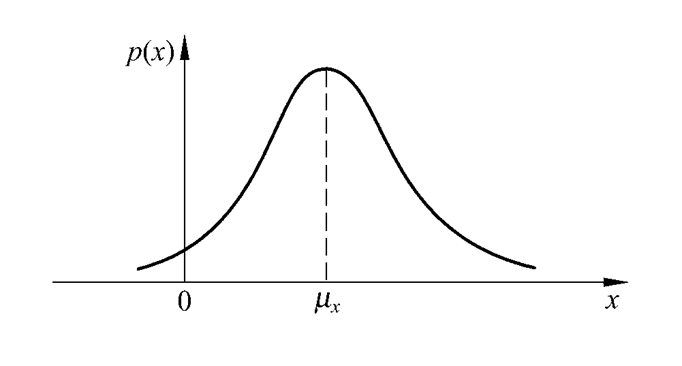
\includegraphics[width=4cm]{Gaussian}\\
		\caption{高斯(正态)分布随机变量的PDF曲线$\mu_x>0$}
	\end{figure}
    \tiny PDF---概率密度函数(Probability Density Function)
\end{columns}
\end{frame}

\begin{frame}{标准高斯(正态)分布随机变量}
归一化处理$x(\xi)\sim\mathcal{N}(\mu_x,\sigma_x^2)$为$x(\xi)\sim\mathcal{N}(0,1)$, 令
\[u(\xi)=\frac{x(\xi)-\mu_x}{\sigma_x}\]
有
\[p(x)=\left(\frac{1}{2\pi}\right)^{1/2}\exp\left(-\frac{u^2}{2}\right) \]
\begin{columns}
\column{0.4\textwidth}%<1->
\begin{figure}[!h]
	\centering
	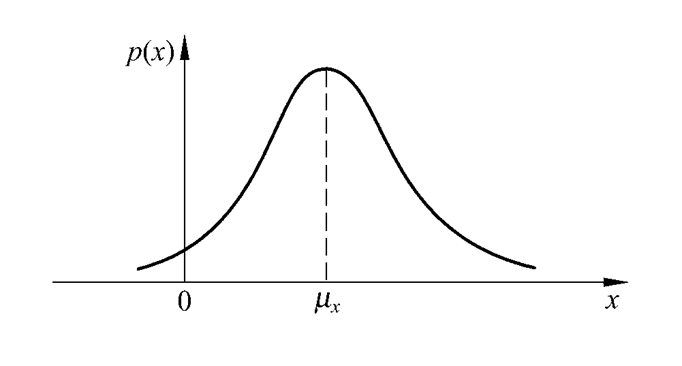
\includegraphics[width=4cm]{Gaussian}\\
	\caption{高斯(正态)分布随机变量的PDF曲线$\mu_x>0$}
\end{figure}
\column{0.4\textwidth}
\begin{figure}[!h]
	\centering
	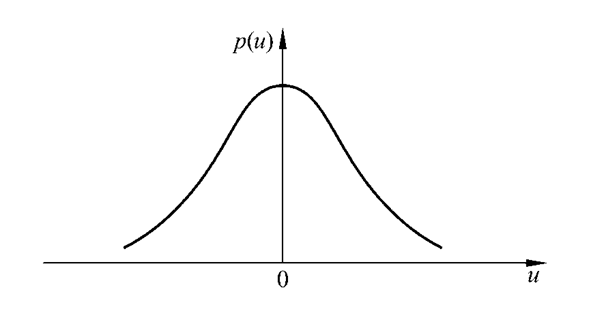
\includegraphics[width=4cm]{GaussianN}\\
	\caption{标准高斯(正态)分布随机变量的PDF曲线$\mu_x>0$}
\end{figure}
\end{columns}
\end{frame}

\begin{frame}{标准高斯(正态)分布随机变量}
\begin{columns}
\column{0.6\textwidth}%<1->
标准高斯分布随机变量的一维累积分布函数(正态概率积分)定义为
\[\Phi(x)\mathop{=}^{def}\int_{-\infty}^{x}\left(\frac{1}{2\pi}\right)^{1/2}\exp\left(-\frac{u^2}{2}\right)du \]
它的互补累积分布函数是标准高斯分布的右尾积分,即
\[Q(x)=1-\Phi(x)\mathop{=}^{def}\int_{x}^{\infty}\left(\frac{1}{2\pi}\right)^{1/2}\exp\left(-\frac{u^2}{2}\right)du \]
\column{0.4\textwidth}
\begin{figure}[!h]
\centering
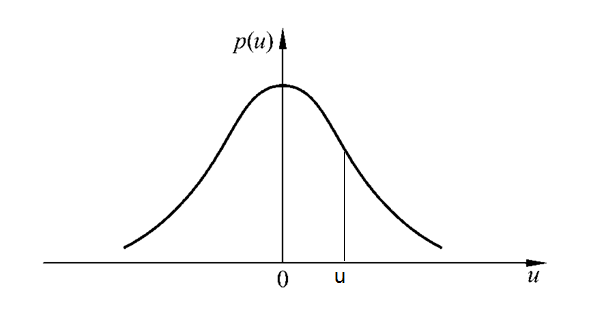
\includegraphics[width=4cm]{GaussianNQ}\\
\caption{标准高斯(正态)分布随机变量的PDF曲线$\mu_x>0$}
\end{figure}
\end{columns}
\end{frame}


\begin{frame}{中心极限定理}
\begin{block}{高斯噪声的数学模型---中心极限定理}
在一般条件下, $N$个相互\textbf{统计独立}的随机变量$n_i$之和$n=\sum\limits_{k=1}^{N}n_k$, 在$N\to\infty$的极限情况下,其概率密度趋于高斯分布,而不管每个变量$n_k$的具体分布如何。
\end{block}
\begin{block}{注}
	(1) 实际上,只要$N$足够大,每个分量之间也不一定完全统计独立,但不存在占统治地位的若干分量,则它们和的分布就可以近似为高斯分布。\\
	(2) 无限多的、相互独立的、各自作用有限的系统干扰分量叠加形成噪声干扰,并且服从高斯分布。
\end{block}
\end{frame}

\begin{frame}{高斯噪声的统计描述(1)}
\begin{definition}[高斯噪声]
	噪声$n(t)$, 对任意$N\ge 1$和所有时刻$t_k$, 随机变量$n(t_k)$服从高斯分布,则$n(t)$为一个高斯噪声随机变量过程,简称高斯噪声过程或高斯噪声。
\end{definition}
\begin{block}{高斯噪声一维概率密度函数}
	\[p(n_k;t_k)=(\frac{1}{2\pi\sigma_{n_k}^2})^{1/2}\exp\left[-\frac{(n_k-\mu_{n_k})^2}{2\sigma_{n_k}^2}\right] \]
	其中,$\mu_{n_k}$为$n(t_k)$的均值, $\sigma_{n_k}$为$n(t_k)$的方差。
\end{block}
\end{frame}

\begin{frame}{高斯噪声的统计描述(2)}
\begin{block}{高斯噪声N维联合概率密度函数}
高斯噪声的N维矢量记为
\[(\bm{n;t})=(n(t_1),n(t_2),\cdots,n(t_N))^T \]
其N维联合概率密度函数为
\begin{align*}
p(\bm{n;t})&=p(n_1,n_2,\cdots,n_N; t_1,t_2,\cdots,t_N)\\
&=\frac{1}{(2\pi)^{N/2}|\bm{C_n}|^{1/2}}\exp\left[-\frac{1}{2}(\bm{n-\mu_n})^T\bm{C_n}^{-1}(\bm{n-\mu_n})\right]
\end{align*}

其中,$\bm{\mu_{n}}$是高斯随机矢量$(\bm{n;t})$的均值矢量,$\bm{C_n}$为协方差矩阵。
即
$$\bm{\mu_n}=(\mu_{n_1},\mu_{n_2},\dots,\mu_{n_N})^T$$
$$\mu_{n_k}=E[n(t_k)]$$
\end{block}
\end{frame}

\begin{frame}
$\bm{C_n}$是高斯随机矢量$\bm{(n;t)}$的协方差
$$
\bm{C_n}=\left[
\begin{matrix}
C_{n_1n_1} & C_{n_1n_2} & \cdots &C_{n_1n_N} \\
C_{n_2n_1} & C_{n_2n_2} & \cdots &C_{n_2n_N} \\
\vdots     &  \vdots    &        &\vdots \\
C_{n_Nn_1} & C_{n_Nn_2} & \cdots &C_{n_Nn_N} \\
\end{matrix}
\right]
$$
其中$C_{n_jn_k}=E[(n(t_j)-\mu_{n_j})(n(t_k)-\mu_{n_k})]=c_{n_k}c_(n_j)$\\
$|\bm{C_n}|$是$\bm{C_n}$的行列式,$\bm{C_n^{-1}}$是$\bm{C_n}$的逆矩阵。
\end{frame}

\begin{frame}{高斯变量$n(t_k)$互不相关$\Leftrightarrow$相互统计独立}
	\begin{block}{不相关性与统计独立性}
		互不相关$\nRightarrow$相互统计独立。但是若$x(t)$服从联合高斯分布,则互不相关$\Leftrightarrow$相互统计独立
	\end{block}
\textbf{证明:} 设高斯随机矢量$\bm{(n;t)}$中的$n(t_j)$与$n(t_k)(j\ne k)$互不相关,即$C_{n_jn_k}=C_{n_kn_j}=0(j\ne k)$, 若记$\sigma_{n_k}^2\mathop{=}\limits^{def}C_{n_kn_k}$,则协方差矩阵$C_n$和$\bm{C_n^{-1}}$分别为
	\begin{columns}
		\column{0.5\textwidth}
		$$
		\bm{C_n}=\left[
		\begin{matrix}
		\sigma_{n_1}^2 &  0                 & \cdots & 0\\
		0              &  \sigma_{n_2}^2  & \cdots & 0\\
		\vdots         &  \vdots            &        &\vdots \\
		0              &  0                 & \cdots &\sigma_{n_N}^2\\
		\end{matrix}
		\right]
		$$
		\column{0.5\textwidth}
		$$\bm{C_n^{-1}}=\left[
		\begin{matrix}
		(\sigma_{n_1}^2)^{-1} &  0                 & \cdots & 0\\
		0              &  (\sigma_{n_2}^2)^{-1}  & \cdots & 0\\
		\vdots         &  \vdots            &        &\vdots \\
		0              &  0                 & \cdots &(\sigma_{n_N}^2)^{-1}\\
		\end{matrix}
		\right]
		$$
	\end{columns}
	而$|\bm{C_n}|^{1/2}$为: $|\bm{C_n}|^{1/2}=\prod\limits_{k=1}^{N}\sigma_{n_k}$
\end{frame}

\begin{frame}
	因此,高斯噪声$n(t)$的N维联合概率密度函数为
	\begin{align*}
	p(\bm{n;t})&=p(n_1,n_2,\cdots,n_N; t_1,t_2,\cdots,t_N)\\
	&=\frac{1}{(2\pi)^{N/2}|\bm{C_n}|^{1/2}}\exp\left[-\frac{1}{2}(\bm{n-\mu_n})^T\bm{C_n}^{-1}(\bm{n-\mu_n})\right]\\
	&=\frac{1}{(2\pi)^{N/2}|\prod\limits_{k=1}^{N}\sigma_{n_k}}\exp\left[-\sum\limits_{k=1}^{N}\frac{(n_k-\mu_{n_k})^2}{2\sigma_{n_k}^2}\right]\\
	&=\prod\limits_{k=1}^{N}\left(\frac{1}{2\pi\sigma_{n_k}}\right)^{1/2}\exp\left[-\frac{(n_k-\mu_{n_k})^2}{2\sigma_{n_k}^2}\right]\\
	&=p(x_1;t_1)p(x_2;t_2)\cdots p(x_N;t_N)
	\end{align*}
	表明$n(t)$的N维联合概率密度函数表示成各自一维概率密度函数之积的形式,即是统计独立性的定义。因此,N个高斯随机变量$n(t_k)(k=1,2,\dots,t_N)$互不相关$\Rightarrow$相互统计独立; 结合之前的结论``相互统计独立的随机变量$\Rightarrow$互不相关''。所以, \textbf{
	N个高斯随机变量$n(t_k)(k=1,2,\dots,t_N)$互不相关$\Leftrightarrow$相互统计独立}。
\end{frame}

\begin{frame}{高斯随机变量的线性组合}
\begin{enumerate}
	\item 若$x_k(\xi)\sim\mathcal{N}(\mu_{x_k},\sigma_{x_k}^2)(k=1,2,\dots,N)$,且它们相互统计独立,则它们的和
	\[x(\xi)=\sum\limits_{k=1}^{N}x_k(\xi) \]
	是高斯随机变量,且有$x_k(\xi)\sim\mathcal{N}(\mu_x,\sigma_x^2)$,其中
	$\mu_x=\sum\limits_{k=1}^N\mu_{x_k},\sigma_x^2=\sum\limits_{k=1}^N\sigma_{x_k}^2$
	\item 更一般地,任意有限N个高斯随机变量$x_k(\xi)(k=1,2,\dots,N)$的线性组合
	\[x(\xi)=\sum\limits_{k=1}^{N}a_kx_k(\xi) \]
	仍然是高斯随机变量,且有$x_k(\xi)\sim\mathcal{N}(\mu_x,\sigma_x^2)$,其中
	$\mu_x=\sum\limits_{k=1}^Na_k\mu_{x_k},\sigma_x^2=\sum\limits_{j=1}^N\sum\limits_{k=1}^Na_ja_kc_{x_kx_j}$\\
	式中,协方差函数$c_{x_jx_k}=E[(x_j(\xi)-\mu_{x_j})(x_k(\xi)-\mu_{x_k})]=c_{x_kx_j},\mu_{x_k}=E[x_k(\xi)]$
\end{enumerate}
\end{frame}

\begin{frame}{白噪声}
\small
%白噪声的频域,时域描述:
\begin{columns}%0.6 0.4表示相对比例
	\column{0.6\textwidth}
	\begin{block}{频域---白噪声的功率谱密度}
	功率谱密度均匀分布在整个频率轴上: $p_n(\omega)=\frac{N_0}{2},\quad -\infty<\omega< \infty, N_0$是常数\\
	也可以按正半轴上的频域定义: $p_n(\omega)=N_0,\quad 0<\omega<\infty, N_0$是常数
	\end{block}
    \column{0.3\textwidth}
    \includegraphics[scale=0.3]{WhiteNoise2}
\end{columns}

\begin{columns}%0.6 0.4表示相对比例
	\column{0.6\textwidth}
	\begin{block}{时域---白噪声的自相关函数}
	均值为零、自相关函数$r_n(\tau)$为$\delta$的噪声随机过程: $r_n(\tau)=IFT[\frac{N_0}{2}]=\frac{N_0}{2}\delta(\tau)$
	\end{block}
	\column{0.3\textwidth}
	\includegraphics[scale=0.3]{WhiteNoise1}
\end{columns}
\begin{block}{意义}
	白噪声是一种理想化的数学模型,由于其功率谱密度在整个频域上均匀分布,所以其能量是无限的,实际上是不存在的。但是由于我们所采用的系统相对于整个频率轴来说是窄带系统,只要认为频谱是均匀分布的,能够在数学上带来很大方便。
\end{block}
\end{frame}

\begin{frame}{白噪声特性}
\includegraphics[scale=0.4]{WhiteNoise}
\begin{block}{白噪声$n(t)$重要特性}
	\begin{itemize}
		\item 白噪声在频域上其功率谱密度是均匀分布的;
		\item 时域上自相关函数$r_n(\tau)$是$\delta$函数: $r_n(\tau)=IFT[\frac{N_0}{2}]=\frac{N_0}{2}\delta(\tau)$
		\item 任意两个不同时刻的随机变量$n(t_j)$与$n(t_k),(\tau=t_j-t_k\ne 0)$是不相关的:\\
		$r_n(t_j,t_k)=r_n(\tau)=E[n(t_j)n(t_k)]=0,(\tau=t_j-t_k\ne 0)$。
		\item 由于$\delta$---函数的筛选性: $\int_{-\infty}^{\infty}\delta(t-t_0)f(t)dt=f(t_0)$,有\\
		$\int_{-\infty}^{\infty}r_n(t-t_0)f(t)dt=f(t_0)=\frac{N_0}{2}\int_{-\infty}^{\infty}\delta(t-t_0)f(t)dt=\frac{N_0}{2}f(t_0)$
	\end{itemize}	
\end{block}
\end{frame}

\begin{frame}{高斯白噪声}
\begin{block}{高斯白噪声$n(t)$重要特性---高斯随机变量+白噪声}
	\begin{itemize}
		\item 高斯白噪声在频域上其功率谱密度是均匀分布的;
		\item \textbf{时域上概率密度函数是高斯分布的。(白噪声对此没有明确限制)}
		\item 时域上自相关函数$r_n(\tau)$是$\delta$函数: $r_n(\tau)=IFT[\frac{N_0}{2}]=\frac{N_0}{2}\delta(\tau)$
		\item 任意两个不同时刻的随机变量$n(t_j)$与$n(t_k),(\tau=t_j-t_k\ne 0)$是不相关的,\textbf{并且是统计独立的}:\\
		$r_n(t_j,t_k)=r_n(\tau)=E[n(t_j)n(t_k)]=0,(\tau=t_j-t_k\ne 0)$。
		\item 由$\delta$---函数的筛选性: $\int_{-\infty}^{\infty}\delta(t-t_0)f(t)dt=f(t_0)$,有\\
		$\int_{-\infty}^{\infty}r_n(t-t_0)f(t)dt=f(t_0)=\frac{N_0}{2}\int_{-\infty}^{\infty}\delta(t-t_0)f(t)dt=\frac{N_0}{2}f(t_0)$
	\end{itemize}	
\end{block}
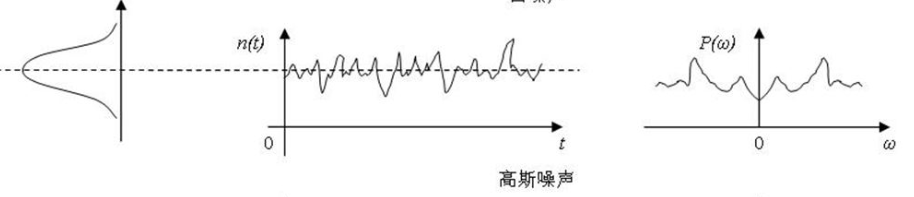
\includegraphics[scale=0.4]{WhiteGaussianNoise}
\end{frame}

\begin{frame}{有色噪声}
如果噪声过程$n(t)$的功率谱密度在频域上的分布是不均匀的,则称其为有色噪声。
\begin{block}{有色噪声的功率谱密度}
	\[P_n(f) =P_0\exp\left[-\frac{(f-f_0)^2}{2\sigma_f^2}\right]\]
	均值$f_0$代表频谱的中心频率,方差$\sigma_f^2$反映噪声的谱宽度。$\omega=2\pi f$
\end{block}
\end{frame}

\begin{frame}[shrink]
\frametitle{ch2.信号检测与估计理论的基础知识}
\tableofcontents[hideallsubsections]
\end{frame}


